\section{Controladores de posición y trayectoria}
\label{sec:posicion}

Una decisión de diseño del proyecto fue conservar la cascada PID de bajo
nivel, que es suficiente para la actitud, y comparar las técnicas avanzadas
\emph{encima} de ella, en el lazo de posición. El simulador tiene cinco controladores con una interfaz común, siete
generadores de trayectoria, un procedimiento de identificación de los
rezagos que los controladores basados en modelo necesitan y un banco de
comparación con métricas sobre la posición verdadera.

\subsection{Interfaz común y restricciones compartidas}

Todos los controladores heredan \cod{PositionController} y corren en el lazo
externo (100~Hz):
\begin{equation}
\texttt{update}(t,\ \text{NavState},\ \text{trayectoria})\ \to\ (\vect a_{des},\ \psi_{ref},\ \dot\psi_{ff})\ \ [\text{u opcionalmente } (T,\phi,\theta,\psi)].
\end{equation}
\cod{NavState} contiene solo cantidades \emph{estimadas} (posición y
velocidad del filtro de navegación, actitud del AHRS, tasas filtradas y la
aceleración cinemática estimada $\vect a_{kin,E}$ de \eqref{eq:akin}) y la
masa \emph{nominal}: el controlador no sabe si alguien le colgó una carga.
La aceleración deseada pasa por la planitud diferencial de la
\cref{sec:planitud}; solo el NMPC entrega empuje y actitud directamente.

Para que la comparación sea justa, PID, MPC y NMPC comparten la misma caja de
aceleraciones admisibles (\cod{common.accel\_limits}):
\begin{equation}
|a_x|,|a_y|\le g\tan30^\circ=\val{axyMax}~\text{m/s}^2,\qquad
-0.8\Big(\frac{T_{max}}{m}-g\Big)=-\val{aUp}\ \le a_z\le\ 0.8\,g=\val{aDown}~\text{m/s}^2 .
\label{eq:caja}
\end{equation}
El factor 0.8 deja un 20~\% de empuje al lazo de actitud: los motores no
pueden dar a la vez todo el empuje y todo el momento (\cref{sec:propulsion}).
El PID acota la norma horizontal en lugar de cada eje, y la política de RL
proyecta sobre un cono de $30^\circ$ con $a_z\in[-6,6]$~m/s$^2$; las tres
formas coinciden en la inclinación máxima en hover sostenido.

\subsection{Generadores de trayectoria}

Cada trayectoria (\cod{trajectories.py}) entrega la referencia y sus tres
primeras derivadas \emph{analíticas}, $(\vect p,\vect v,\vect a,\vect j)$,
más el rumbo. Los controladores las usan como prealimentación y el MPC y el
NMPC como previsión del horizonte. Hay siete: vuelo estacionario,
escalones (caja en XY más escalón de altura), círculo, figura en 8, hélice,
mínimo \emph{snap} por puntos de paso y punto a punto de mínimo
\emph{jerk}.

\paragraph{Arranque desde el reposo.} Una curva periódica pura, por ejemplo
$x=R\cos\omega t$, arranca con velocidad $R\omega$: un escalón en la
referencia de velocidad que ningún dron puede seguir y que contaminaría las
métricas con un transitorio arbitrario. Las curvas periódicas se recorren
con una fase $\vartheta(t)$ cuya velocidad sube con el polinomio
\emph{smoothstep} de quinto orden,
\begin{equation}
\dot\vartheta=\omega\,s\!\left(\frac{t}{T_r}\right),\qquad s(u)=10u^3-15u^4+6u^5,
\label{eq:smooth}
\end{equation}
que cumple $s(0)=0$, $s(1)=1$ y $s'=s''=0$ en ambos extremos. Por la regla
de la cadena,
\begin{equation}
\vect v=\vect f'\dot\vartheta,\quad
\vect a=\vect f''\dot\vartheta^2+\vect f'\ddot\vartheta,\quad
\vect j=\vect f'''\dot\vartheta^3+3\vect f''\dot\vartheta\ddot\vartheta+\vect f'\dddot\vartheta,
\end{equation}
y en $t=0$ velocidad, aceleración y \emph{jerk} son exactamente cero (el
bloque M lo verifica: $\max|\cdot|=0$). Como $\int_0^1s=1/2$, la rampa recorre
media vuelta equivalente; con la rampa simétrica de bajada la trayectoria
termina en reposo en el punto de partida tras un número entero de vueltas,
y dura $n_{vueltas}T+T_r$.

\paragraph{Figura en 8.} Lemniscata de Gerono en el plano horizontal,
\begin{equation}
x=c_x+A\sin\vartheta,\qquad y=c_y+\tfrac{B}{2}\sin2\vartheta,
\label{eq:gerono}
\end{equation}
con $A=2$~m y $B=1$~m (el 8 mide $4\times1$~m). Es la prueba clásica de
seguimiento en la literatura de MPC para cuadricópteros
\cite{torrente21,sun22}, aunque esos trabajos la usan a velocidades mucho
mayores y con otra parametrización; la de Gerono se eligió por su forma
cerrada. Con periodo de 10~s (dos vueltas) alcanza \val{lemV}~m/s y
\val{lemA}~m/s$^2$ (inclinación de \val{lemTilt}$^\circ$); la versión rápida
del banco, con periodo de 5~s y tres vueltas, \val{lemRV}~m/s y
\val{lemRA}~m/s$^2$, que exigen \val{lemRTilt}$^\circ$ de inclinación, cerca del
límite de 30$^\circ$. El círculo de 1.5~m y 10~s llega a \val{cirV}~m/s.

\paragraph{Mínimo snap.} Para recorrer puntos de paso, Mellinger y Kumar
\cite{mellinger11} minimizan $\int\|\vect p^{(4)}\|^2dt$. Por
Euler--Lagrange la solución cumple $\vect p^{(8)}=0$ en cada tramo:
polinomios de grado 7. Con la asignación de tiempos fija
($T_i=\max(t_{min},d_i/\bar v)$), posiciones impuestas en los puntos de
paso, reposo ($v=a=j=0$) en los extremos y continuidad de las derivadas 1 a
6 en los puntos interiores, el número de ecuaciones iguala al de incógnitas
($8M$ para $M$ tramos) y la solución del sistema lineal \emph{es} el mínimo
\cite{richter13}. Cada tramo usa tiempo normalizado $\tau\in[0,1]$ para que
la matriz esté bien condicionada. Verificación: el salto relativo de las
derivadas 1--6 en los nudos es \val{msJump}.

\subsection{Identificación de los rezagos del lazo interno}
\label{sec:identificacion}

Visto desde el lazo de posición, todo lo que hay debajo (planitud, AHRS,
cascada de actitud, mezclador, motores) es un sistema
$\vect a_{des}\to\vect a$. Los controladores basados en modelo necesitan
una descripción simple de él. \cod{identification.py} la obtiene con un
ensayo de escalón sobre el simulador \emph{completo}, como en un banco
real: el dron arranca en hover, un comandante en lazo abierto aplica un
escalón $+U$ y, en otra corrida con la misma semilla, $-U$; la semidiferencia
cancela la deriva común (sesgos, ruido). Sobre esa respuesta se ajusta por
mínimos cuadrados
\begin{equation}
y(t)=K\,U\left(1-e^{-(t-\theta)/\tau}\right),\quad t>\theta,
\label{eq:fopdt}
\end{equation}
con búsqueda en malla sobre $(\theta,\tau)$ y $K$ lineal en cada punto, en
dos versiones: primer orden con retardo (FOPDT) y primer orden puro
($\theta=0$, que absorbe el retardo en $\tau$ por la regla de la mitad).

\begin{table}[H]
\centering
\small
\caption{Rezagos identificados del PAE-X450 que usan los controladores
(\cod{DEFAULT\_LAGS}; identificados con Madgwick y el núcleo anterior,
escalones de 1.5~m/s$^2$ y $8^\circ$). Error RMS relativo del ajuste entre
paréntesis.}
\label{tab:lags}
\begin{tabular}{lcc}
\toprule
Canal & Primer orden puro & FOPDT \\
\midrule
$a_{des,xy}\to a_{xy}$ & $\tau_{a,xy}=\val{tauAxy}$~ms (\val{rmseFO}~\%) & $\val{tauAxyF}$~ms $+$ \val{thAxyF}~ms (\val{rmseFOPDT}~\%) \\
$a_{des,z}\to a_z$ & $\tau_{a,z}=\val{tauAz}$~ms (\val{rmseZ}~\%) & igual, sin retardo \\
$\phi_{ref}\to\phi$ & $\tau_{att}=\val{tauAtt}$~ms & $\val{tauAttF}$~ms $+$ \val{thAttF}~ms \\
\bottomrule
\end{tabular}
\end{table}

\begin{figure}[H]
\centering
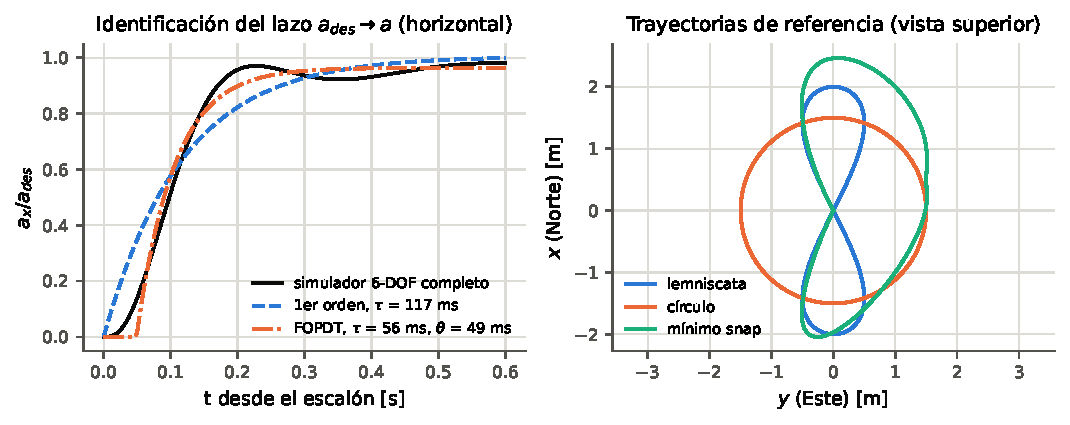
\includegraphics[width=\textwidth]{identificacion_trayectorias.pdf}
\caption{Izquierda: respuesta del simulador completo a un escalón de
aceleración horizontal y los dos ajustes. Derecha: figura en 8, círculo y
trayectoria de mínimo snap por defecto (vista superior).}
\label{fig:ident}
\end{figure}

La lectura de la \cref{fig:ident} es importante para entender los resultados
del banco. El lazo horizontal no es de primer orden: es de segundo orden,
con una curva en S, una joroba hacia los 0.2~s y una cola lenta que deja el
integrador del lazo de tasa. El primer orden puro de 119~ms comete un 7.5~\%
de error; el FOPDT, 3.1~\%. El canal vertical, en cambio, es casi
exactamente el motor ($T_m=20$~ms). Todos los controladores basados en
modelo comparten ese error de modelado.

La \cref{tab:lags} es la que usan los controladores, y se identificó con el
núcleo anterior. El ensayo de la \cref{fig:ident} se repitió con el núcleo
actual (estimador \val{estDef}, acelerómetro filtrado, $k_d=K_c\theta$,
giroscopio a 60~Hz; bloque M): el canal horizontal da
$\tau=\val{reidTau}$~ms como primer orden puro (\val{reidRmseFO}~\% de error)
y $\val{reidTauF}~\text{ms}+\val{reidThF}~\text{ms}$ como FOPDT
(\val{reidRmseFOPDT}~\%). \cod{DEFAULT\_LAGS} no se regeneró tras el cambio
del núcleo.

\subsection{PID en cascada (estilo PX4)}

\cod{position/pid.py} reproduce la estructura de \cod{mc\_pos\_control} de
PX4: un P de posición que genera una referencia de velocidad, y un PID de
velocidad con prealimentación de la velocidad y la aceleración de
referencia:
\begin{align}
\vect v_{sp}&=\vect v_{ref}+\sat_{v_{max}}\!\big(K_p(\vect p_{ref}-\hat{\vect p})\big),\qquad
\vect e_v=\vect v_{sp}-\hat{\vect v},\nonumber\\
\vect a_{des}&=\sat_{\text{caja}}\Big(\vect a_{ref}+K_v\vect e_v+K_i\!\int\!\vect e_v\,dt+K_d\,\tfrac{d}{dt}\vect e_v\Big),
\label{eq:pidpos}
\end{align}
con la corrección de velocidad acotada ($3$~m/s en XY, $2$~m/s en $z$),
integración condicional e integral acotada como en \eqref{eq:pid}, y el
derivativo filtrado a 5~Hz (apagado por defecto, $K_d=0$). Sin
prealimentación un lazo de posición solo corrige \emph{después} de que el
error aparece.

\paragraph{Ganancias derivadas del modelo.} Con las mismas reglas SIMC de
la \cref{sec:control} sobre la planta identificada: el lazo de velocidad ve
$a_{cmd}\to v=1/s$ con el FOPDT de la \cref{tab:lags}, y la regla de la mitad
da $\theta_{ef}=\tau+\theta+\Delta t/2$ ($\Delta t/2$ es la retención del lazo
de 100~Hz). Con $\tau_c=\max(1.5\,\theta_{ef},\,0.1~\text{s})$, más
conservador que el ``ajustado'' $\tau_c=\theta$ para dejar margen al ruido del
estimador,
\begin{equation}
K_v=\frac{1}{\tau_c+\theta_{ef}},\quad K_i=\frac{K_v}{4(\tau_c+\theta_{ef})},\quad
K_p=\frac{1}{3\,(\tau_c+\theta_{ef})}.
\end{equation}
Resulta $K_p=\val{pdkpxy}$, $K_v=\val{pdkvxy}$, $K_i=\val{pdkixy}$ en XY y
$K_p=\val{pdkpz}$, $K_v=\val{pdkvz}$, $K_i=\val{pdkiz}$ en $z$; los valores por
defecto de PX4 son todavía más conservadores (0.95 / 1.8 / 0.4 en XY).

\paragraph{Ganancias afinadas en simulación.} Para el PAE-X450, $K_p$ y $K_v$
salen de una malla $K_p\in\{2.4,3,3.6,4.5\}\times K_v\in\{4.5,5.5,6.5\}$ con
$K_i=K_v^2/4$ (la relación SIMC $T_i=4/K_v$), escogiendo el mínimo del RMSE
medio en figura en 8 y círculo: $K_p=3.6$, $K_v=5.5$, $K_i=7.56$, que bajó el
RMSE de 6.2 a 3.1~cm frente a las ganancias derivadas (malla hecha con el
núcleo anterior y Madgwick, escenario nominal, semilla 1). El MPC y el NMPC
se afinaron con el mismo protocolo. Esa semilla es también una de las tres
del banco final, y el integral se eligió mirando el caso con interferencia
magnética (nota siguiente): los tres controladores clásicos se afinaron
sobre parte del conjunto de prueba, cosa que no se hizo con el RL
(\cref{sec:banco}). Es, en pequeño, el flujo que propone el proyecto: sintonía en
simulación como punto de partida. El valor por defecto actual del integral
es, sin embargo, $K_{i,xy}=\val{pidKiDef}$, por la razón de la nota
siguiente: el óptimo en el escenario nominal no es el óptimo robusto.

\begin{nota}[Fragilidad del integral con interferencia magnética]
Las cifras de esta nota son anteriores a restringir la corrección magnética
al rumbo (\cref{sec:estimadores}); el banco final de la \cref{sec:banco} ya
incluye ese cambio. Con EMI en el magnetómetro el rumbo estimado se desviaba 11--12$^\circ$; el
empuje real queda rotado respecto de la aceleración pedida, y un integral
grande sobre una planta rotada entra en espiral. Con el núcleo actual
(Mahony, acelerómetro filtrado), en la figura en 8 nominal $K_{i,xy}=2$ dio
2.35~cm de RMSE frente a 2.38~cm con 7.56; con EMI, 4.99~cm frente a 73~cm
(semilla 1, medido antes de corregir el desfase de 10~ms del registro de la
referencia que se explica en la \cref{sec:banco}; el orden de magnitud de la
diferencia no depende de esa corrección).
Por eso el valor por defecto pasó a 2.0. Aun así, con EMI y
\emph{escalones} de 1~m el PID entra en un ciclo límite saturado en la
inclinación máxima: es un hallazgo del banco, no un error de
implementación. El MPC, cuyo observador de perturbación estima la
aceleración no explicada en lugar de integrar el error, no lo sufre.
\end{nota}

\subsection{MPC lineal con previsión}

\paragraph{Modelo de predicción.} Por eje, desacoplado, con la aceleración
total como estado y el rezago identificado (\cod{position/mpc.py}):
\begin{equation}
\dot p=v,\qquad \dot v=a,\qquad \dot a=\frac{u-a}{\tau_a},\qquad
\vect x=[p,v,a]\T,\ u=a_{cmd},
\label{eq:mpc_model}
\end{equation}
con $\tau_a=\tau_{a,xy}$ en $x,y$ y $\tau_{a,z}$ en $z$. Se discretiza de
forma \emph{exacta} con retención de orden cero y paso $h=\Delta t_{pred}$;
con $\alpha=e^{-h/\tau}$ y $\beta=1-\alpha$:
\begin{equation}
A=\begin{bmatrix}1&h&\tau(h-\tau\beta)\\0&1&\tau\beta\\0&0&\alpha\end{bmatrix},\qquad
B=\begin{bmatrix}h^2/2-\tau h+\tau^2\beta\\ h-\tau\beta\\ \beta\end{bmatrix}.
\label{eq:zoh}
\end{equation}
El bloque M compara \eqref{eq:zoh} con la exponencial de la matriz aumentada
(\cod{scipy.linalg.expm}) para tres $\tau$ y dos pasos: error máximo
\val{zohErr}.

\paragraph{Costo.} Sobre un horizonte de $N=20$ pasos de 50~ms (1~s), con la
referencia muestreada en $t+kh$:
\begin{equation}
J=\sum_{k=1}^{N}q_p(p_k-p_{ref,k})^2+q_v(v_k-v_{ref,k})^2
+\sum_{k=0}^{N-1}r_u\,(u_k-u_{ref,k})^2+r_{du}(u_k-u_{k-1})^2 .
\label{eq:mpc_cost}
\end{equation}
La entrada de referencia es la que hace que el modelo con rezago siga
exactamente la aceleración de referencia: si $a=a_{ref}$, entonces
$u_{ref}=a_{ref}+\tau_a\,j_{ref}$, evaluada en el centro de cada intervalo.
Con $u_{ref}=0$ el término $r_uu^2$ sesgaría el seguimiento hacia
aceleración nula (en un círculo, hacia adentro); penalizando la
\emph{desviación} el sesgo desaparece. Pesos por defecto: $q_p=1$, $q_v=0$
en XY; $q_{pz}=2$, $q_{vz}=0.1$; $r_u=5\times10^{-4}$, $r_{du}=0$.

\paragraph{QP condensado y su solución.} Eliminando los estados con
$\vect p=\Phi\vect x_0+\Gamma\vect U$, el costo es una cuadrática en las $N$
entradas, $\tfrac12\vect U\T H\vect U+\vect f\T\vect U$, con
$H=2(q_p\Gamma_p\T\Gamma_p+q_v\Gamma_v\T\Gamma_v+r_uI+r_{du}D\T D)$ precalculada y
$\vect f$ lineal en el estado y en la previsión. Las únicas restricciones son
la caja \eqref{eq:caja} sobre $\vect U$, así que la proyección es exacta y
barata. El algoritmo: (1) se calcula el óptimo sin restricciones
$\vect U^*=-H^{-1}\vect f$; si cumple la caja, es el óptimo exacto (caso más
común en el banco). (2) Si no, FISTA \cite{beck09} con reinicio por
gradiente \cite{odonoghue15}, precondicionado diagonal (Jacobi:
$\tilde H=SHS$, $S=\diag(H)^{-1/2}$), paso $1/L$ con $L=\lambda_{max}(\tilde H)$,
arranque en caliente con la solución anterior desplazada y un máximo de 60
iteraciones. Con ese tope el costo queda a menos del 0.3~\% del óptimo y el
tiempo medio es de 0.4~ms por llamada.

\paragraph{Estado no medido y acción libre de offset.} La aceleración no se
mide: se usa la predicción del modelo interno, la última entrada aplicada
filtrada por el mismo rezago,
$a_{lag}\leftarrow e^{-\Delta t/\tau}a_{lag}+(1-e^{-\Delta t/\tau})u_{apl}$. Para
rechazar perturbaciones constantes (viento medio, carga, error de empuje)
se agrega un observador de Luenberger de perturbación de entrada
(\cod{common.DisturbanceObserver}) sobre el modelo $\dot v=a_{lag}+d$,
$\dot d=0$, con la velocidad estimada como medida:
\begin{equation}
\hat v\leftarrow\hat v+\Delta t\,\big(a_{lag}+\hat d+\ell_1(v-\hat v)\big),\qquad
\hat d\leftarrow\hat d+\Delta t\,\ell_2(v-\hat v),\qquad
s^2+\ell_1s+\ell_2=s^2+2\zeta\omega s+\omega^2,
\label{eq:dob}
\end{equation}
con $\omega=3$~rad/s y $\zeta=0.8$ (polos en $-2.4\pm1.8j$). Es el esquema
``offset-free'' de Pannocchia y Rawlings \cite{pannocchia03} y Maeder,
Borrelli y Morari \cite{maeder09}: $\hat d$ absorbe todo lo que el modelo no
explica. El QP trabaja con la aceleración total $a=a_{lag}+\hat d$ y la
entrada desplazada $\tilde u=u+\hat d$; se aplica
$u=\sat_{\text{caja}}(\tilde u_0-\hat d)$.

\paragraph{Ley equivalente.} Sin restricciones activas el MPC es una ley
lineal en el estado y en la previsión (\cod{lq\_gain}). Para el eje $x$,
$u_0=-\val{mpcKx}\,(p-p_{ref})-\val{mpcKvx}\,v-\val{mpcKax}\,a+(\text{términos de previsión})$;
la suma de las ganancias de posición y de previsión es \val{mpcInv} (debe ser
cero por invarianza a traslaciones). Comparada con el PID afinado (rigidez
$K_pK_v=19.8$~s$^{-2}$, amortiguamiento $K_v=5.5$~s$^{-1}$), el MPC es casi
el doble de rígido y además se anticipa: ve venir la curva un segundo antes.

\subsection{MPC no lineal (iLQR con restricciones de caja)}

\paragraph{Modelo de predicción.} Nueve estados y tres entradas
(\cod{position/nmpc.py}):
\begin{gather}
\vect x=[\vect p,\vect v,\phi,\theta,T],\qquad \vect u=[T_c,\phi_c,\theta_c],\nonumber\\
\dot{\vect p}=\vect v,\quad
\dot{\vect v}=g\eu-\frac{T}{m}\,\vect r_3(\phi,\theta,\psi)-\frac{c_d}{m}\vect v|\vect v|+\hat{\vect d},\quad
\dot\phi=\frac{\phi_c-\phi}{\tau_{att}},\quad
\dot\theta=\frac{\theta_c-\theta}{\tau_{att}},\quad
\dot T=\frac{T_c-T}{\tau_T},
\label{eq:nmpc}
\end{gather}
con $\vect r_3=\R\eu=(c_\phi s_\theta c_\psi+s_\phi s_\psi,\ c_\phi s_\theta s_\psi-s_\phi c_\psi,\ c_\phi c_\theta)$
la tercera columna de la matriz Z-Y-X, $\psi$ el rumbo de referencia
(exógeno), $\tau_{att}=\val{tauAtt}$~ms y $\tau_T=\tau_{a,z}$ de la
\cref{tab:lags}. Es genuinamente no lineal: proyección trigonométrica del
empuje sin aproximar, producto $T\vect r_3$ y arrastre cuadrático (aplicado en
$\E$, supuesto; la planta lo aplica en $\B$, y la diferencia la absorbe
$\hat{\vect d}$).

\paragraph{Discretización.} Los tres estados de rezago son lineales y se
integran exactamente con ZOH; $(\vect p,\vect v)$ con un paso RK4 que evalúa
el rezago en $0,h/2,h$. Un RK4 sobre los nueve estados quedaría al borde de
su región de estabilidad: con $h=50$~ms y $\tau_T=19.5$~ms, $h/\tau_T=2.6$,
cerca del límite de 2.785 en el eje real, y su factor de amplificación por
paso para ese modo sería 0.75 frente al exacto $e^{-2.6}=0.07$.

\paragraph{Costo y referencia.} Cuadrático en el error de posición y
velocidad y en la desviación de las entradas respecto de una referencia
$\vect u_{ref}$ que sale de la planitud diferencial
(\cref{sec:planitud}) aplicada a $\vect a_{ref}+\tau_{att}\vect j_{ref}-\hat{\vect d}+\frac{c_d}{m}\vect v_{ref}|\vect v_{ref}|$,
con peso terminal. Restricciones de caja:
$T_c\in[\val{nmpcTlo},\val{nmpcThi}]$~N (la misma caja vertical del MPC) y
$|\phi_c|,|\theta_c|\le30^\circ$.

\paragraph{Solver.} iLQR \cite{li04,tassa12} con entradas acotadas a la
manera de \emph{box-DDP} \cite{tassa14}. Los jacobianos $A_k,B_k$ se calculan
por diferencias finitas, todos los pasos del horizonte en un solo lote
vectorizado. En el paso hacia atrás, con
$Q_{uu}=\ell_{uu}+B_k\T V_{xx}B_k+\mu I$ y $Q_{ux}=B_k\T V_{xx}A_k$, se
comprueba con Cholesky que $Q_{uu}$ sea definida positiva; si no lo es,
$\mu$ se multiplica por 10 y se repite el paso (regularización adaptativa de
Levenberg--Marquardt, \cite{tassa12}), y tras un paso exitoso vuelve a bajar.
Con jacobianos por diferencias finitas, $V_{xx}$ puede perder la definición
positiva en saturación o ante perturbaciones grandes. Luego se
resuelve en cada $k$ el QP de caja de dimensión 3 para la corrección
$\delta\vect u_k$ por Newton proyectado, y las filas de la ganancia
$K_k=-Q_{uu}^{-1}Q_{ux}$ de las entradas que quedaron en su cota se anulan
(no hay realimentación en una dirección saturada). El paso hacia adelante
simula en lote los candidatos $\alpha\in\{1,0.5,0.25,0\}$,
$\vect u_k=\sat(\vect U_k+\alpha\,\delta\vect u_k+K_k(\hat{\vect x}_k-\vect X_k))$, y
se queda con el de menor costo; $\alpha=0$ es el despliegue en lazo cerrado
del arranque en caliente, así que el costo nunca empeora. Se hace una
iteración por llamada con arranque en caliente (iteración en tiempo real,
\cite{diehl05}); el costo medido en la máquina de desarrollo es de
3.8~ms de mediana por llamada
(\cod{experiments/nmpc\_timing.py}), y depende mucho del procesador y de la
versión de Python y numpy: otra máquina midió 16~ms. Las pruebas de tiempo
de cómputo, por esa razón, no corren por defecto.

\paragraph{Por qué no supera al MPC lineal.} Medido en la figura en 8
rápida (con el núcleo anterior y Madgwick): con 1, 2 o 3 iteraciones el RMSE apenas cambia (5.24, 5.15,
5.20~cm), de modo que el optimizador no es el límite; quitando el arrastre
del modelo tampoco empeora. Hasta unos $16^\circ$ de inclinación la
proyección trigonométrica es casi lineal, y ambos comparten el error de
modelo dominante: el lazo de actitud real es de segundo orden con unos
43~ms de retardo, no un primer orden (\cref{fig:ident}).

\subsection{Aprendizaje por refuerzo puro (PPO fuera de línea)}

El requisito de diseño fue no entrenar nunca un RL sobre una planta lenta:
entrenar fuera de línea en un entorno rápido, después transferir y validar.
El simulador 6-DOF corre a unas 10 veces el tiempo real; PPO necesita del
orden de $10^7$ pasos, que en el 6-DOF serían horas por millón. Por eso el
flujo (detallado en \cod{docs/RL.md}) fue el siguiente. Las políticas se
entrenaron con el núcleo anterior (sustituto identificado con Madgwick) y
\emph{no se reentrenaron} tras las correcciones; en el banco final actúan
sobre el núcleo actual sin cambios, lo que es en sí una prueba adicional de
transferencia.

\begin{enumerate}
\item \textbf{Sustituto identificado.} Solo la traslación, con el lazo
interno como retardo más primer orden por eje y la masa real distinta de
la nominal,
\begin{equation}
\vect a_{thr}=\frac{e^{-d s}}{\tau s+1}\,\vect a_{des},\qquad
\vect a=g\eu+\frac{m_{nom}}{m}\big(\vect a_{thr}-g\eu\big)-\frac{c_d}{m}\vect v_r|\vect v_r|,\quad \vect v_r=\vect v-\vect v_w,
\label{eq:surrogate}
\end{equation}
identificado con escalones aleatorios sobre el 6-DOF (núcleo anterior,
Madgwick, 30~s). Hubo dos identificaciones. La política pura se entrenó con
la primera, hecha antes de inicializar bien el estimador:
$\tau_{xy}=90$~ms, $d=28$~ms ($R^2=0.951$ del ajuste horizontal;
\cod{experiments/results/rl/surrogate\_id\_v1\_used\_for\_pure.json}). El
híbrido se entrenó con la corregida: $\tau_{xy}=82.5$~ms, $d=32$~ms
($R^2=0.982$ en el ajuste y 0.981 en datos de validación;
\cod{models/surrogate\_id.json}). En ambas, $\tau_z=25$~ms sin retardo, y
las dos caen dentro del rango aleatorizado. Vectorizado en numpy, 128
entornos en paralelo.
\item \textbf{Aleatorización de dominio} \cite{tobin17}: masa
($\times0.85$--$1.20$), carga a mitad de episodio, $\tau$ ($\pm30$~\%),
retardo (10--50~ms), arrastre ($\pm50$~\%), viento medio hasta 5~m/s,
turbulencia de Gauss--Markov, ráfagas $1-\cos$ y ruido de medida. La
política no observa ninguno de estos parámetros.
\item \textbf{MDP.} Paso de 10~ms (el lazo externo), episodios de 10~s.
Observación de 24 componentes con escalas fijas: errores de posición y
velocidad \emph{estimados}, velocidad y aceleración de referencia,
previsión de la referencia a 0.25 y 0.5~s, última acción y una integral con
fugas del error de posición ($\dot I=e_p-I/3$~s). Acción
$\vect a_{des}=\operatorname{proy}_{30^\circ}(6~\text{m/s}^2\cdot\pi(\vect o))$.
Recompensa $r=-\min(c,25)$ con
$c=w_{pl}\|e_p\|+w_p\|e_p\|^2+w_v\|e_v\|^2+w_a\|\vect a-\vect a_{ref}\|^2+w_{da}\|\Delta\vect a\|^2$
sobre errores \emph{verdaderos} (información privilegiada, legítima solo
porque el entrenamiento es fuera de línea).
\item \textbf{PPO} \cite{schulman17} con actor y crítico de $2\times64$
neuronas tanh, GAE, recorte 0.2, 50~M de pasos (33~min).
\item \textbf{Validación Sim2Sim}: la política corre sin reentrenar en el
6-DOF completo, con el mismo banco que los demás controladores.
\end{enumerate}

Dos aclaraciones para leer los resultados. El círculo y la figura en 8 son
casos particulares de la familia de referencias de entrenamiento (multiseno
con una componente por eje), y la figura en 8 rápida queda en su borde: la
validación mide interpolación, no generalización. Y la comparación no es
simétrica en el diseño: el RL ve 0.5~s de previsión (el MPC, 1~s, con
velocidad y prealimentación de referencia), con escalas fijas sin
normalizar, una salida que no está estructurada como corrección sobre
$\vect a_{ref}$, y un límite de inclinación en cono de $30^\circ$ frente a la
caja por eje de \eqref{eq:caja}, que en diagonal admite algo más. Hubo un
solo entrenamiento PPO (semilla 0), cortado cuando la curva todavía bajaba.

\subsection{Híbrido MPC + RL residual}

El híbrido suma al MPC lineal real una corrección aprendida
\cite{johannink19,silver18}:
\begin{equation}
\vect a_{des}=\sat_{\text{caja}}\big(\vect a_{MPC}+s\,R\,\pi(\vect o)\big),\qquad R=2~\text{m/s}^2,\ s\in[0,1.5],
\label{eq:residual}
\end{equation}
donde la observación agrega la acción del MPC y su perturbación estimada
(30 componentes) y $s=0$ recupera el MPC exacto. Después de sumar el
residuo se le informa al MPC la entrada realmente aplicada, para que su
modelo de rezago y su observador no confundan el residuo con una
perturbación externa y lo cancelen. La red se entrenó con el MPC replicado
dentro del entorno sustituto, y el punto guardado fue el de menor
\emph{costo} de evaluación. Como el costo premia el esfuerzo y la suavidad
además del error, ese criterio eligió una red que empeora el seguimiento ya
en el sustituto: en la figura en 8 nominal sin aleatorizar, MPC+RL da
0.48~cm de RMSE frente a 0.14~cm del MPC solo, y durante el entrenamiento
de la variante suave el costo bajó de 0.070 a 0.040 mientras el RMSE de
evaluación subía de 5.28 a 5.72~cm (\cod{docs/RL.md}).

\subsection{Banco de comparación}
\label{sec:banco}

\cod{experiments/benchmark\_controllers.py} corre controladores
$\times$ trayectorias $\times$ escenarios $\times$ semillas con la misma
inicialización (\cod{scenarios.prepare\_tracking\_sim}), el mismo
estimador y el mismo bajo nivel, y calcula las métricas de \cod{metrics.py}
sobre la posición \emph{verdadera}: RMSE por eje y 3D, error máximo, IAE,
ITAE, esfuerzo (RMS de $\|u\|$ del lazo de actitud, el mismo actuador para
todos), porcentaje de tiempo con el mezclador desaturando y, en la
trayectoria de escalones, tiempo de subida, sobreimpulso y
establecimiento. La \cref{tab:banco} es el banco final con el núcleo
corregido (\cod{experiments/results/benchmark\_final}): los cinco
controladores, \val{bancoNTraj} trayectorias (\val{bancoTrajList}), los cuatro escenarios
de la \cref{sec:perturbaciones} y las semillas \val{bancoSeedList}, con el
estimador \val{estDef}: \val{bancoN} combinaciones y \val{bancoVuelos}
vuelos simulados.

\begin{nota}[Alineación temporal de la referencia en el registro]
El error de seguimiento se calcula como $\vect p(t)-\vect p_{ref}(t)$ con
ambos evaluados en el mismo instante. Una auditoría independiente encontró
que versiones anteriores del registro guardaban la referencia de la última
llamada del lazo externo, hasta 10~ms más vieja que la posición; a 1.4~m/s
eso son 1.4~cm de error ficticio en la dirección de avance. Ahora
\cod{Simulation.\_log} y \cod{telemetry} evalúan la referencia en el instante
del estado (\cod{\_ref\_now}). La corrección bajó todas las métricas de
seguimiento (en la figura en 8, semilla 1: MPC de 1.99 a 1.37~cm, PID de
2.35 a 1.70~cm) y hace que las cifras de bancos anteriores, incluidas las de
\cod{docs/RL.md} y \cod{docs/BARRIDOS.md}, no sean comparables con las de
esta tabla.
\end{nota}

\begin{table}[H]
\centering
\small
\caption{Banco final: RMSE 3D [cm], media $\pm$ desviación estándar
muestral ($n=\val{bancoSeeds}$ semillas, ddof $=1$); estimador \val{estDef},
núcleo corregido. La negrita marca solo la media más baja de cada fila; la
\cref{sec:lectura_banco} explica qué se puede afirmar con estas semillas.}
\label{tab:banco}
\setlength{\tabcolsep}{2.6pt}
\begin{tabular}{llccccc}
\toprule
Trayectoria & Escenario & PID & MPC & NMPC & RL puro & MPC+RL \\
\midrule
\val{bancoRows}
\midrule
\multicolumn{2}{l}{Cómputo por llamada} & \val{bancoComp} \\
\bottomrule
\end{tabular}
\end{table}

\begin{figure}[H]
\centering
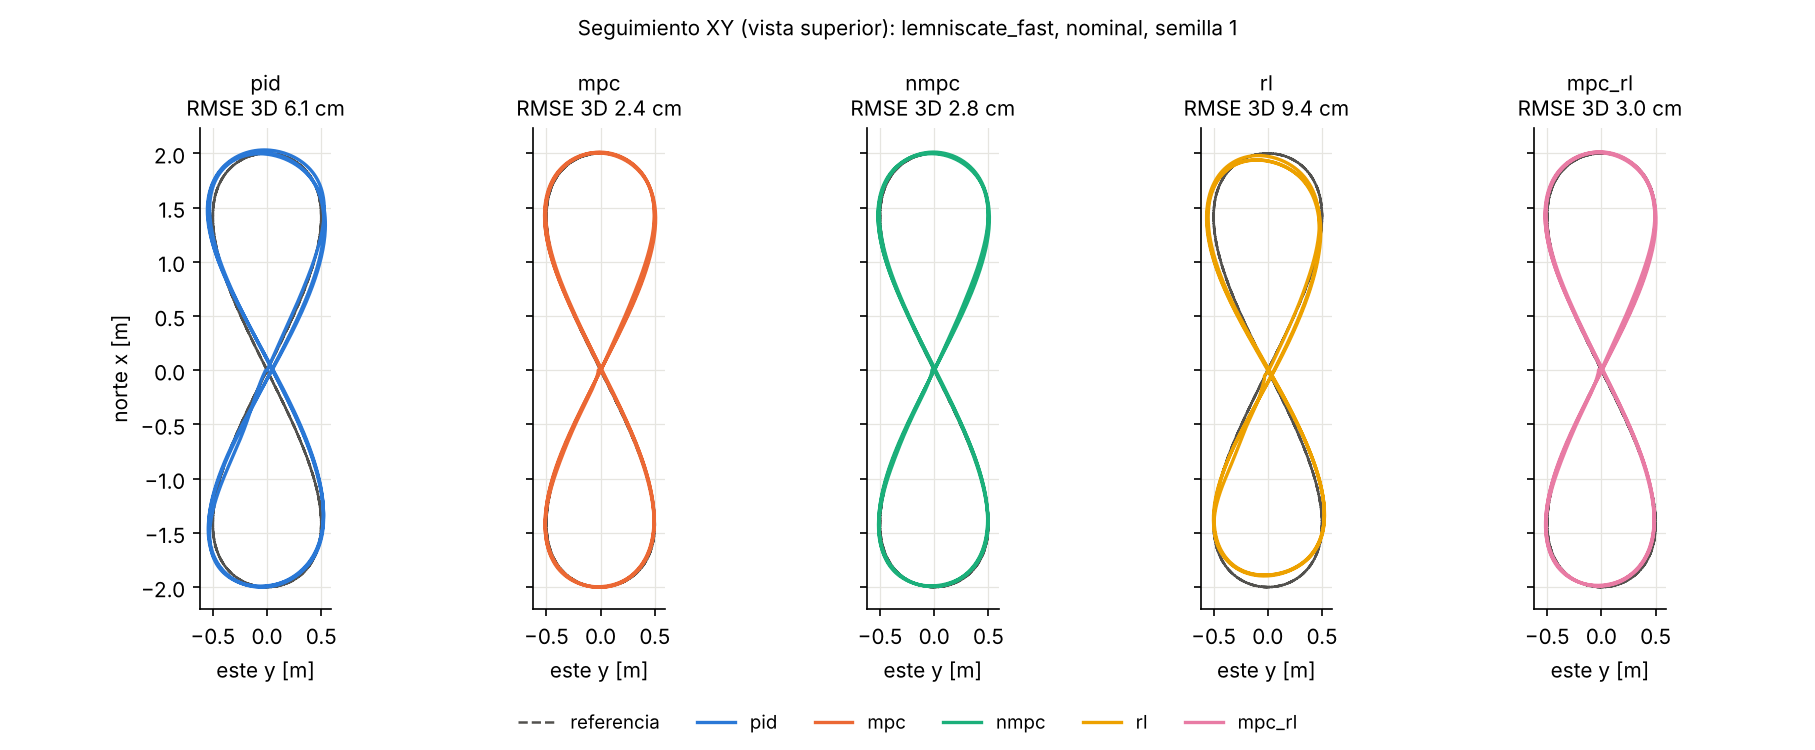
\includegraphics[width=\textwidth]{xy_lemniscate_fast_nominal.png}
\caption{Figura en 8 rápida, escenario nominal, semilla 1: trayectoria
horizontal de los cinco controladores sobre la referencia (banco final).}
\label{fig:xy}
\end{figure}

\begin{figure}[H]
\centering
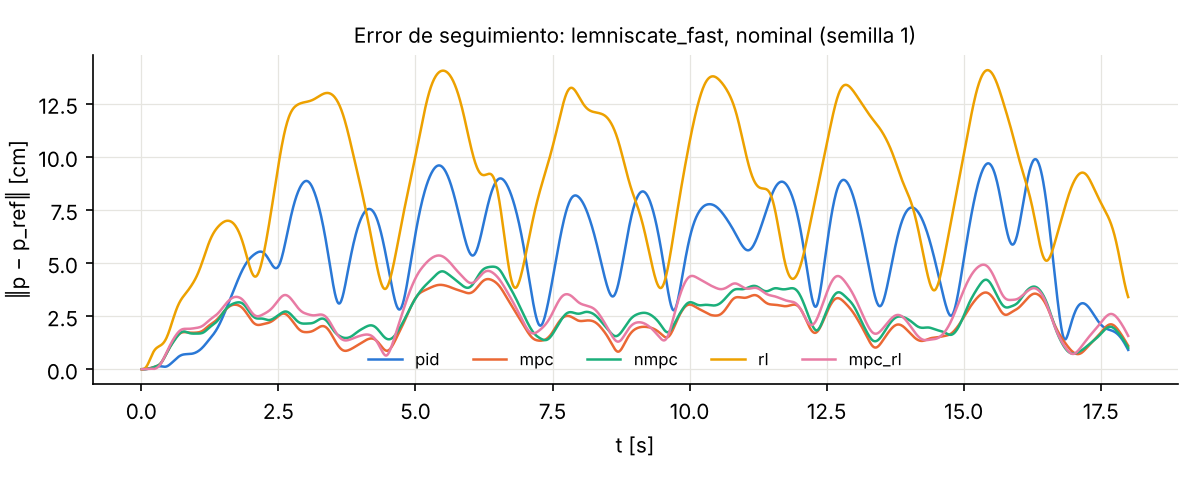
\includegraphics[width=\textwidth]{err_lemniscate_fast_nominal.png}
\caption{Norma del error de posición en la figura en 8 rápida, escenario
nominal, semilla 1 (banco final).}
\label{fig:err}
\end{figure}

\begin{table}[H]
\centering
\small
\caption{Trayectoria de escalones (caja de 1~m en XY y escalón de altura),
escenario nominal: métricas de escalón horizontal promediadas sobre los
escalones y las tres semillas. ``n/d'': no queda dentro de la banda del
2~\% antes del siguiente escalón.}
\label{tab:escalones}
\begin{tabular}{lccccc}
\toprule
 & PID & MPC & NMPC & RL puro & MPC+RL \\
\midrule
Sobreimpulso [\%] & \val{bpidstepwaypointsnominalos} & \val{bmpcstepwaypointsnominalos} & \val{bnmpcstepwaypointsnominalos} & \val{brlstepwaypointsnominalos} & \val{bmpcrlstepwaypointsnominalos} \\
Subida 10--90~\% [s] & \val{bpidstepwaypointsnominaltr} & \val{bmpcstepwaypointsnominaltr} & \val{bnmpcstepwaypointsnominaltr} & \val{brlstepwaypointsnominaltr} & \val{bmpcrlstepwaypointsnominaltr} \\
Establecimiento 2~\% [s] & \val{bpidstepwaypointsnominalts} & \val{bmpcstepwaypointsnominalts} & \val{bnmpcstepwaypointsnominalts} & \val{brlstepwaypointsnominalts} & \val{bmpcrlstepwaypointsnominalts} \\
Error final [cm] & \val{bpidstepwaypointsnominalss} & \val{bmpcstepwaypointsnominalss} & \val{bnmpcstepwaypointsnominalss} & \val{brlstepwaypointsnominalss} & \val{bmpcrlstepwaypointsnominalss} \\
\bottomrule
\end{tabular}
\end{table}

\subsection{Lectura del banco}
\label{sec:lectura_banco}

\paragraph{Qué permiten afirmar tres semillas.} En las filas de figura en 8
y círculo los rangos $\pm$ de MPC, NMPC y MPC+RL se solapan, de modo que la
tabla, leída columna contra columna, no separa a esos tres. La comparación
útil es por semilla, porque cada semilla da a todos los controladores el
mismo ruido, el mismo sesgo y la misma turbulencia. Con ese criterio el MPC
queda por debajo del PID en \val{pairMpcPid} de las \val{pairTotal} parejas
(fila $\times$ semilla) y por debajo del NMPC en todas las semillas de
\val{pairMpcNmpcRows} de las \val{nCombos} filas; el MPC+RL queda por
encima del MPC en \val{pairMpcrlWorse} de las \val{pairTotal}. Aun cuando
las tres semillas coinciden, una prueba de signos da $p=0.25$ (bilateral):
son tendencias consistentes, no diferencias estadísticamente probadas. Para
probarlas harían falta más semillas. Hay además un detalle de cálculo: la
validación de \cod{docs/RL.md} usó la desviación poblacional y este banco
la muestral, así que sus $\pm$ no se comparan directamente.

\paragraph{Controladores clásicos.} El MPC lineal tiene la media más baja en
\val{bestMpc} de las \val{nCombos} filas y el NMPC en \val{bestNmpc}. En la
figura en 8 rápida nominal el MPC reduce el error del PID en
\val{fastGain}~\%, porque anticipa la referencia en lugar de reaccionar a
ella. El NMPC cuesta unas \val{nmpcCost} veces más cómputo que el MPC sin
mejorarlo en las trayectorias suaves, por las razones de la sección
anterior. Hay que recordar la asimetría de la afinación: PID, MPC y NMPC se
afinaron con la semilla 1 de la figura en 8 y el círculo, que forma parte
de esta tabla.

\paragraph{Interferencia magnética en maniobra rápida.} Es la fila más
exigente del banco. \val{lostSentence} Los demás la sostienen, y su
resultado depende de una decisión de diseño del filtro de navegación. La
compuerta de innovación (\cref{sec:estimadores}) rechaza una medida de
posición solo si es improbable (más de 5 desviaciones estándar) \emph{y}
además grande (más de 25~cm, \cod{gate\_min\_m}). Con la interferencia, el
rumbo estimado se desvía y el acelerómetro se lleva al marco inercial con
un rumbo equivocado, así que la predicción del filtro queda sesgada. Frente a
un sensor de posición de 1~cm de ruido, una compuerta puramente estadística
descartaría entonces de forma sistemática medidas correctas y el filtro
derivaría: con ella, el MPC llega a 1.6~m de RMSE en esta fila; con el
piso, a \val{bmpclemniscatefastmagemi}~cm. En las trayectorias lentas con
interferencia la diferencia entre controladores es menor (el PID en la
figura en 8 da \val{bpidlemniscatemagemi}~cm, frente a
\val{bmpclemniscatemagemi}~cm del MPC); con los escalones de 1~m, en cambio,
el PID entra en el ciclo límite descrito antes
(\val{bpidstepwaypointsmagemi}~cm).

\paragraph{Aprendizaje por refuerzo.} El RL puro no alcanza al MPC: en
\val{rlRatioRows}, su RMSE medio va de \val{rlRatioMin} a \val{rlRatioMax}
veces el del MPC, y por semilla llega a \val{rlRatioSeedMax}. Tampoco es
siempre el peor: supera al PID en \val{rlBeatsPid} de las \val{nCombos}
filas (\val{rlBeatsPidList}).

La causa de la brecha está, sobre todo, en la política. En su propio
sustituto, sin aleatorizar, el RL puro ya comete 4.25~cm de RMSE en la
figura en 8, frente a 0.14~cm del MPC (\cod{validation\_gap\_ablation.json},
núcleo anterior); en esta tabla comete \val{brllemniscatenominal}~cm. Casi
todo el error ya existía donde se entrenó, y lo que falta en el
sustituto explica el resto. Cuáles dinámicas faltantes pesan más
(segundo orden del lazo de actitud, acoplamiento, ruido y retardo de la
posición, vibración) es por ahora una hipótesis: la comparación entre
sustituto y 6-DOF cambia todos esos factores a la vez y se hizo con el
núcleo anterior, con un sustituto que hoy, re-identificado, da otros
rezagos ($\approx$75~ms y 40~ms frente a 82.5 y 32~ms). El híbrido
aumenta el RMSE del MPC entre un \val{resMin} y un \val{resMax}~\% según la
fila; como se vio arriba, su residuo ya empeora al MPC dentro del sustituto.
